\documentclass{article}

\usepackage{graphicx}
\usepackage{tikz}
\usepackage{tikzsymbols}
\usetikzlibrary{calc,patterns,shapes.geometric}
\pagestyle{empty}
\usepackage[margin=0pt]{geometry}
\geometry{papersize={14in,12in}}

\def\centerarc[#1](#2)(#3:#4:#5){\draw[#1] ($(#2)+({#5*cos(#3)},{#5*sin(#3)})$) arc (#3:#4:#5);}

\begin{document}
	\begin{figure}
		\centering
		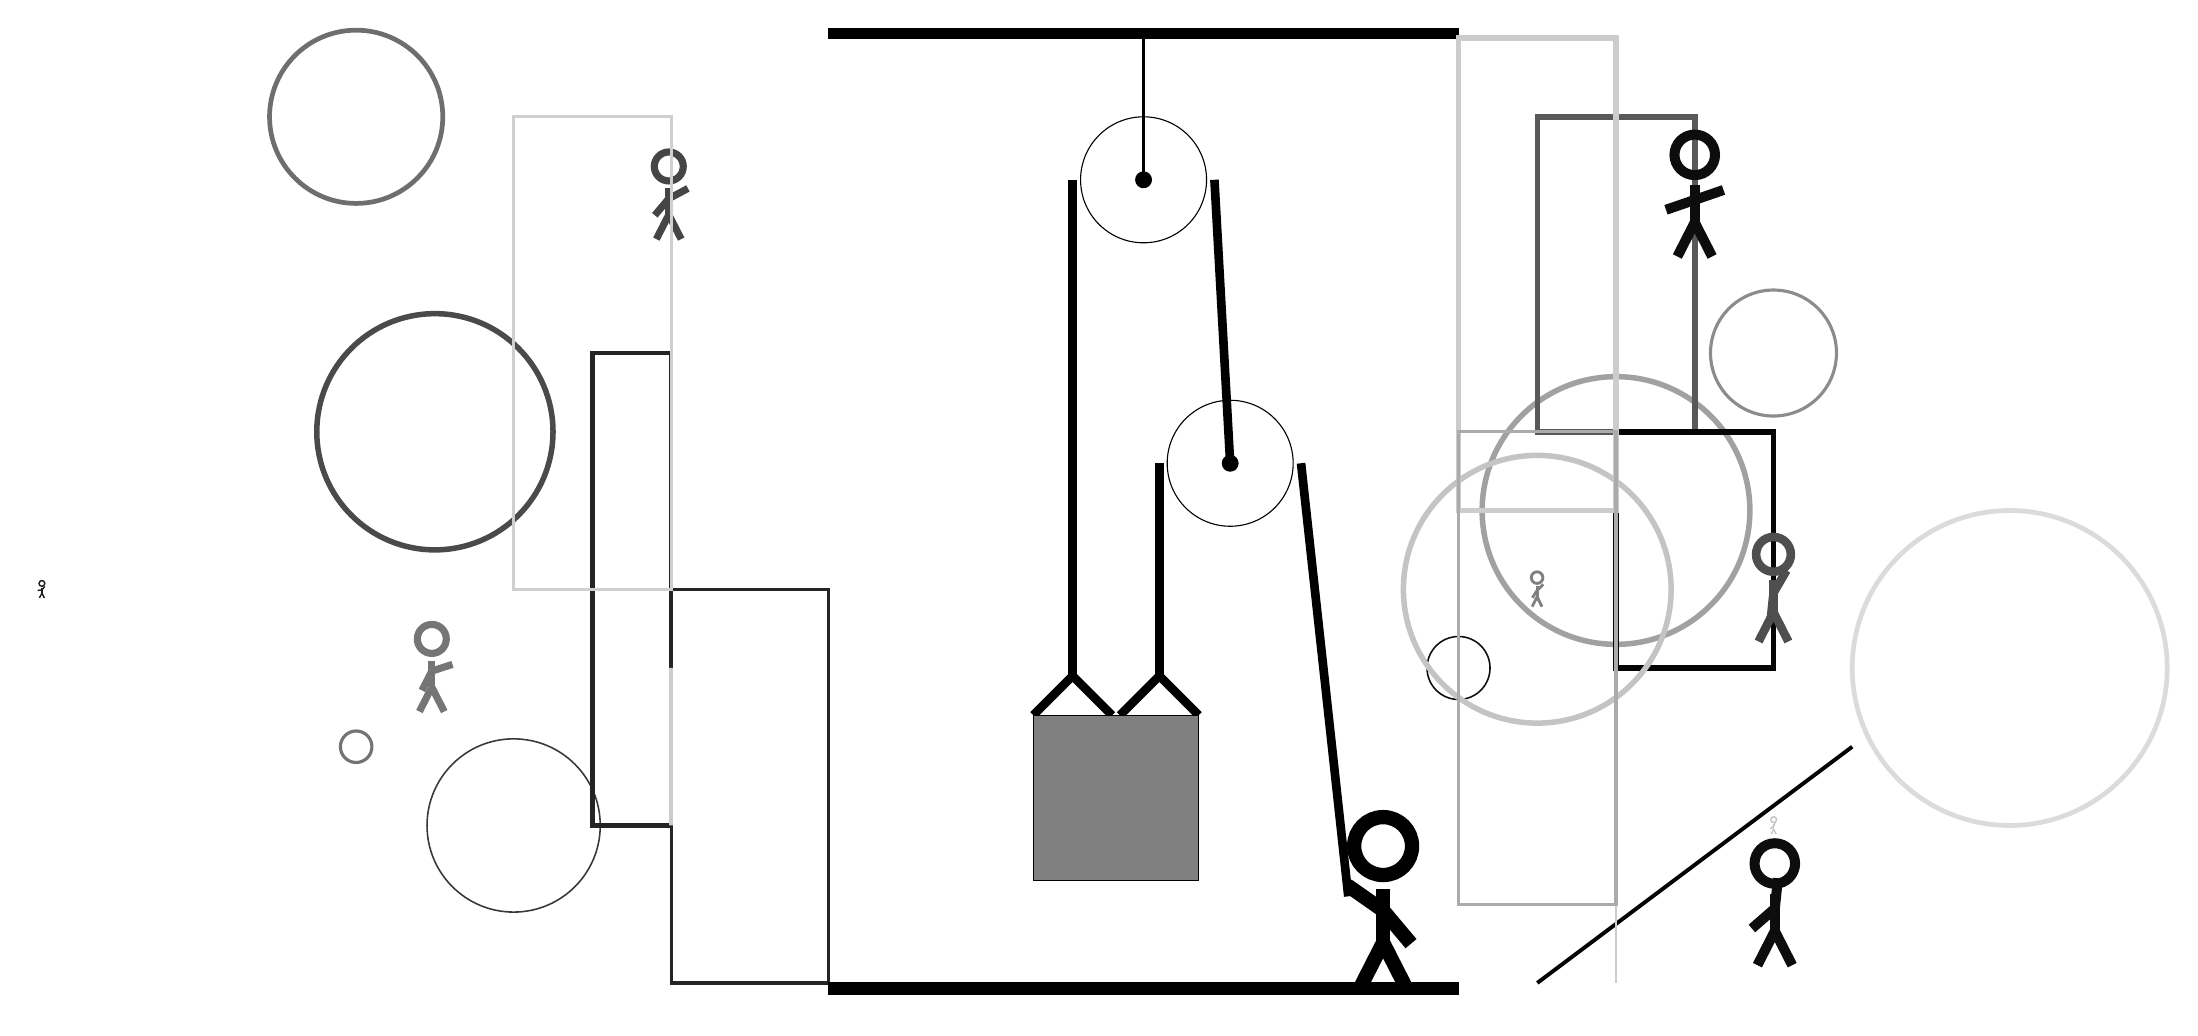
\begin{tikzpicture}
			%%%%% START %%%%%
			
			\draw[fill=black] (-2, 9) rectangle (6, 9.125);
			
			\draw (2, 7.2) circle (0.8);
			\draw[fill=black] (2, 7.2) circle (0.1);
			\draw[thick] (2, 7.2) -- (2, 9);
			
			\draw (3.1, 3.6) circle (0.8);
			\draw[fill=black] (3.1, 3.6) circle (0.1);
			
			\draw [line width=0.7mm, color=black!37](8, 3) circle (1.7);
			
			\draw [line width=0.6mm, color=black!14](13, 1) circle (2.0);
			\node[line width=0.7mm, color=black!88] at (-12, 2) {\Strichmaxerl[1][8][50]};
			\draw[line width=0.5mm, color=black!99](7, -3) -- (11, 0);
			\node[line width=0.3mm, color=black!73] at (-4, 7) {\Strichmaxerl[5][50][28]};
			\draw [line width=0.2mm, color=black!94](6, 1) circle (0.4);
			\draw [line width=0.4mm, color=black!45](10, 5) circle (0.8);
			\draw[line width=0.2mm, color=black!20] (8, -3) rectangle (8, 0);
			\draw[line width=0.7mm, color=black!65] (7, 4) rectangle (9, 8);
			
			\draw[line width=0.7mm, color=black!98] (8, 4) rectangle (10, 1);
			\draw [line width=0.2mm, color=black!78](-6, -1) circle (1.1);
			
			\node[line width=0.7mm, color=black!69] at (10, 2) {\Strichmaxerl[6][84][60]};
			\draw[line width=0.5mm, color=black!50] (6, 6) rectangle (6, 3);
			
			\draw[line width=0.4mm, color=black!85] (-4, -3) rectangle (-2, 2);
			\node[line width=0.5mm, color=black!95] at (10, -2) {\Strichmaxerl[7][41][84]};
			\draw [line width=0.7mm, color=black!71](-7, 4) circle (1.5);
			
			\node[line width=0.6mm, color=black!23] at (10, -1) {\Strichmaxerl[1][41][69]};
			\node[line width=0.5mm, color=black!54] at (-7, 1) {\Strichmaxerl[5][63][18]};
			\draw[line width=0.7mm, color=black!20] (6, 9) rectangle (8, 3);
			\draw [line width=0.6mm, color=black!57](-8, 8) circle (1.1);
			\node[line width=0.2mm, color=black!50] at (7, 2) {\Strichmaxerl[2][57][45]};
			
			\node[line width=0.2mm, color=black!95] at (9, 7) {\Strichmaxerl[7][19][19]};
			
			\draw [line width=0.7mm, color=black!23](7, 2) circle (1.7);
			\draw[line width=0.6mm, color=black!86] (-4, 5) rectangle (-5, -1);
			\draw[line width=0.6mm, color=black!20] (-4, -1) rectangle (-4, 1);
			\draw[line width=0.3mm, color=black!20] (-4, 2) rectangle (-4, 3);
			\draw[line width=0.4mm, color=black!33] (6, -2) rectangle (8, 4);
			\draw [line width=0.4mm, color=black!55](-8, 0) circle (0.2);
			\draw[line width=0.4mm, color=black!19] (-4, 2) rectangle (-6, 8);
			\draw [line width=0.5mm, color=black!60](11, 4) circle (0.0);
			
			\draw[line width = 1.1mm]  (0.6, 0.4) -- (1.1, 0.9) -- (1.6, 0.4);
			\draw[line width = 1.1mm]  (1.7, 0.4) -- (2.2, 0.9) -- (2.7, 0.4);
			\draw[fill=black!50] (0.6, 0.4) rectangle (2.7, -1.7);
			
			\draw[line width = 1.1mm] (1.1, 7.2) -- (1.1, 0.9);
			\centerarc[line width = 1.1mm](2, 7.2)(0:180:0.9);
			\draw[line width = 1.1mm] (2.9, 7.2) -- (3.1, 3.6);
			\draw[line width = 1.1mm] (2.2, 3.6) -- (2.2, 0.9);
			\centerarc[line width = 1.1mm](3.1, 3.6)(0:180:0.9);
			\draw[line width = 1.1mm] (4.0, 3.6) -- (4.6, -1.9);
			
			\node at (5, -2) {\Strichmaxerl[10][-35][-50]};
			
			\draw[fill=black] (-2, -3) rectangle (6, -3.15);
			
			%%%%% END %%%%%
		\end{tikzpicture}
	\end{figure}	
\end{document}